\documentclass[draftspec]{sbmlpkgspec}
\usepackage{microtype}
\usepackage{color}

%% ============================================================================
%% Description:  Documentation for sbmlpkgspec.cls
%% First author: Michael Hucka <mhucka@caltech.edu>
%% Organization: California Institute of Technology
%% Date created: September 2011
%% https://sbml.svn.sourceforge.net/svnroot/sbml/trunk/project/tex/sbmlpkgspec
%%
%% Copyright (C) 2011-2012 California Institute of Technology, Pasadena, CA.
%%
%% SBMLPkgSpec is free software; you can redistribute it and/or modify it
%% under the terms of the GNU Lesser General Public License as published by
%% the Free Software Foundation.  A copy of the license agreement is provided
%% in the file named "LICENSE.txt" included with this software distribution.
%% ============================================================================

% Macros just for this document:

\newcommand{\sbmlpkg}{\texorpdfstring{%
    \textls[-25]{\textsc{SBMLPkgSpec}}}{%
    \textsc{SBMLPkgSpec}}\xspace}
\newcommand{\sbmlpkghead}{\texorpdfstring{%
    \textls[-50]{\textsc{SBMLPkgSpec}}}{%
    \textsc{SBMLPkgSpec}}\xspace}
\newcommand{\sbmlpkgfile}{\literalFont{sbmlpkgspec.cls}\xspace}
\newcommand{\latex}{\LaTeX{}\xspace}
\newcommand{\tex}{\TeX{}\xspace}
\newcommand{\distURL}{http://sourceforge.net/projects/sbml/files/specifications/tex}
\newcommand{\srcURL}{https://sbml.svn.sourceforge.net/svnroot/sbml/trunk/project/tex/sbmlpkgspec}
\newcommand{\webURL}{http://sbml.org/Documents/Specifications/The_SBMLPkgSpec_LaTeX_class}
\newcommand{\cmd}[1]{\literalFont{\textbackslash #1}}

% Custom latex listing style, for use with the listings package.  The default
% highlights far too many things, IMHO.  This keeps it simple and only adjusts
% the appearance of comments within listings.

\lstdefinelanguage{mylatex}{%
  morekeywords={},%
  sensitive,%
  alsoother={0123456789$_},%$
  morecomment=[l]\%%
}[keywords,tex,comments]

\lstdefinestyle{latex}{language=mylatex}


%Listing style for SBOL RDF/XML serialization examples
\usepackage{listings}
\usepackage{color}
\usepackage{xcolor} 
\definecolor{dkgreen}{rgb}{0,0.6,0}
\definecolor{gray}{rgb}{0.5,0.5,0.5}
\definecolor{light-gray}{gray}{0.97}
\lstdefinelanguage{sbol}
    {morekeywords={xmlns:sbol,rdf:about,sbol:displayId,sbol:persistentIdentity,sbol:version,sbol:timeStamp,sbol:name,sbol:description,sbol:member,sbol:Collection,sbol:type, sbol:role, sbol:ComponentDefinition },
     basicstyle=\fontsize{7}{9}\selectfont\ttfamily,
     backgroundcolor=\color{light-gray},
     keywordstyle=\color{blue},
     commentstyle=\color{gray},
     stringstyle=\color{dkgreen},
     tabsize=2,
     showspaces=false,
     showstringspaces=false,
     breaklines=true,                           % wrap text
     sensitive=true,                            % keywords are case sensitive
     %morecomment=[l][commentstyle]{\#},         % comment format
     morestring=[b]",                           % string format
     alsoletter=:
}

%Command to format the listings containing SBOL RDF/XML serialization examples
\newcommand{\lstsetsbol}{
 \lstset{language=sbol,
        tabsize=2
 }
}

%Commands to format SBOL terms in the document
\newcommand{\sbolheading}[1]{\texttt{#1}}
\newcommand{\sbol}[1]{\texttt{\hyperref[sec:#1]{#1}}}

%Command to format external terms in the document
\newcommand{\external}[1]{\texttt{#1}}




% -----------------------------------------------------------------------------
% Start of document
% -----------------------------------------------------------------------------

\begin{document}

\packageTitle{\latex Class for SBML Package Specifications}
\packageVersion{Version 2.0.0}
\packageVersionDate{1 January 2014}

\title{BBF RFC ?: Synthetic Biology Open Language \texorpdfstring{\\[3pt]}{}\mbox{(SBOL) Version~2.0.0}}

\author{Nicholas Roehner\\[0.25em]
  \mailto{nicholasroehner@gmail.com}\\[0.25em]
  Bioengineering\\
  Boston University\\
  Cambridge, MA, USA
}

\maketitlepage
\maketableofcontents

% -----------------------------------------------------------------------------
\section{Purpose}
% -----------------------------------------------------------------------------

% -----------------------------------------------------------------------------
\section{Relation to other BBF RFCs}
% -----------------------------------------------------------------------------

% -----------------------------------------------------------------------------
\section{Copyright Notice}
% -----------------------------------------------------------------------------

% -----------------------------------------------------------------------------
\section{Acknowledgements}
% -----------------------------------------------------------------------------

% -----------------------------------------------------------------------------
\section{Introduction}
% -----------------------------------------------------------------------------

% -----------------------------------------------------------------------------
\section{Overview of SBOL}
% -----------------------------------------------------------------------------
This is some test text. 

% -----------------------------------------------------------------------------
\section{SBOL Vocabulary}
% -----------------------------------------------------------------------------

% -----------------------------------------------------------------------------
\section{SBOL Data Model}
% -----------------------------------------------------------------------------
In this section we describe the major entities of an SBOL document and the relationships between these entities. Complete SBOL examples and best practices when using SBOL can be found in Section \ref{sec:examples} and Section \ref{sec:bestpractices} respectively. 



\subsection {SBOL Document}
Each SBOL document is also a valid RDF/XML document and starts with an XML declaration with the XML version set to "1.0". The top most rdf:RDF XML element includes the SBOL namespace declaration, as shown in the example below. This namespace is used to identify SBOL defined entities and their properties.

\lstsetsbol
\begin{lstlisting}
<?xml version="1.0" ?>
<rdf:RDF xmlns:rdf="http://www.w3.org/1999/02/22-rdf-syntax-ns#" xmlns:sbol="http://sbols.org/v2#">
...
</rdf:RDF>
\end{lstlisting}

An SBOL document can also include custom namespace declarations which are used to embed application specific data as explained in section \ref{sec:annotations}.




\subsection {Identified}
\label{sec:Identified}

\begin{figure}[ht]
\begin{center}
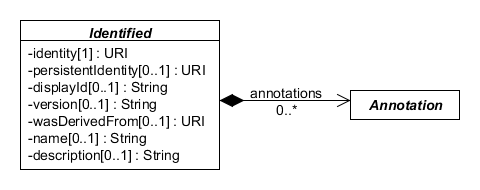
\includegraphics[scale=0.6]{uml/identified}
\caption[]{The Identified class}
\label{uml:identified}
\end{center}
\end{figure}

SBOL-defined classes are all directly or indirectly derived from the Identified abstract class. This inheritance allows SBOL objects to be identified using unique URIs that may refer to relative locations within an SBOL document or permanent URLs from the World Wide Web. This class includes the following properties: \sbol{identity}, \sbol{persistentIdentity}, \sbol{version} and \sbol{timeStamp}
(\ref{uml:identified}).
%TODO: Is there any example SBOL entity that does not derive from Identified?

\subsubsection*{The \sbolheading{identity} property}
\label{sec:identity}
This property is required in all \sbol{Identified} objects and has a datatype of \external{URI}. As before in SBOL Version 1.1, this \external{URI} serves to uniquely identify a SBOL object. The \sbol{identity} attribute can be used to point to other objects from the same SBOL document or resources on the Web. Although all SBOL-defined properties are controlled using the SBOL namespace, this property is represented using the \external{http://www.w3.org/1999/02/22-rdf-syntax-ns\#about} term (see \ref{ser:Collection}).

\subsubsection*{The \sbolheading{persistentIdentity} property}
\label{sec:persistentIdentity}
The \sbol{persistentIdentity} property is optional and also has a datatype of \external{URI}. This property is used to declare that a set of SBOL objects are versions of each other (by virtue of having the same persistent URI). This persistent URI is ideally used to return the most up-to-date version of a SBOL object.

\subsubsection*{The \sbolheading{version} property}
\label{sec:version}
This property has a datatype of \external{String} and is used along with the \sbol{persistentIdentity} property to indicate the current version of an SBOL object.

\subsubsection*{The \sbolheading{timeStamp} property}
\label{sec:timeStamp}
This property has a datatype of \external{TimeStamp} and is used to indicate the creation time of a SBOL object.




\subsection {Documented}
\label{sec:Documented}
The Documented abstract class in SBOL represents objects that can be decorated with human-readable properties, such as name and description. This class extends \sbol{Identified} with three additional data properties: \sbol{displayId}, \sbol{name}, and \sbol{description} (\ref{uml:documented}). 

\begin{figure}[ht]
\begin{center}
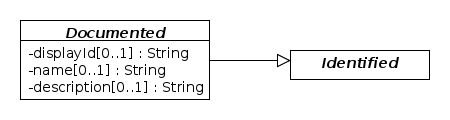
\includegraphics[scale=0.6]{uml/documented}
\caption[]{The Documented class}
\label{uml:documented}
\end{center}
\end{figure}

\subsubsection*{The \sbolheading{displayId} property}
\label{sec:displayId}
An optional display ID, with a data type of \external{String}. It is intended to be used when visualising SBOL objects.

\subsubsection*{The \sbolheading{name} property}
\label{sec:name}
An optional, human readable name property, with a data type of \external{String}. If a \sbol{Documented} object lacks a \sbol{displayId}, it is expected that software tools will instead display the entity's \sbol{name} or \sbol{identity} as a last resort.

\subsubsection*{The \sbolheading{description} property}
\label{sec:description}
An optional, free text description property with the data type of \external{String}.




\subsection {TopLevel}
\label{sec:TopLevel}
\sbol{TopLevel} is an abstract class that is extended by any \sbol{Documented} object that can be found at the top level of a SBOL file, that is any SBOL object that is not nested inside another object when written to a file. Instead of nesting, composite \sbol{TopLevel} objects link to their subordinate \sbol{TopLevel} objects via \external{URI}s when written to a file. For example, a composite \sbol{Component} object A would link to its sub-Component object B using B's \external{URI}. TopLevel classes include \sbol{Sequence}, \sbol{ComponentDefinition}, \sbol{ModuleDefinition}, \sbol{Module}, \sbol{Collection} and \sbol{GenericTopLevel} (\ref{uml:toplevel}).

\begin{figure}[ht]
\begin{center}
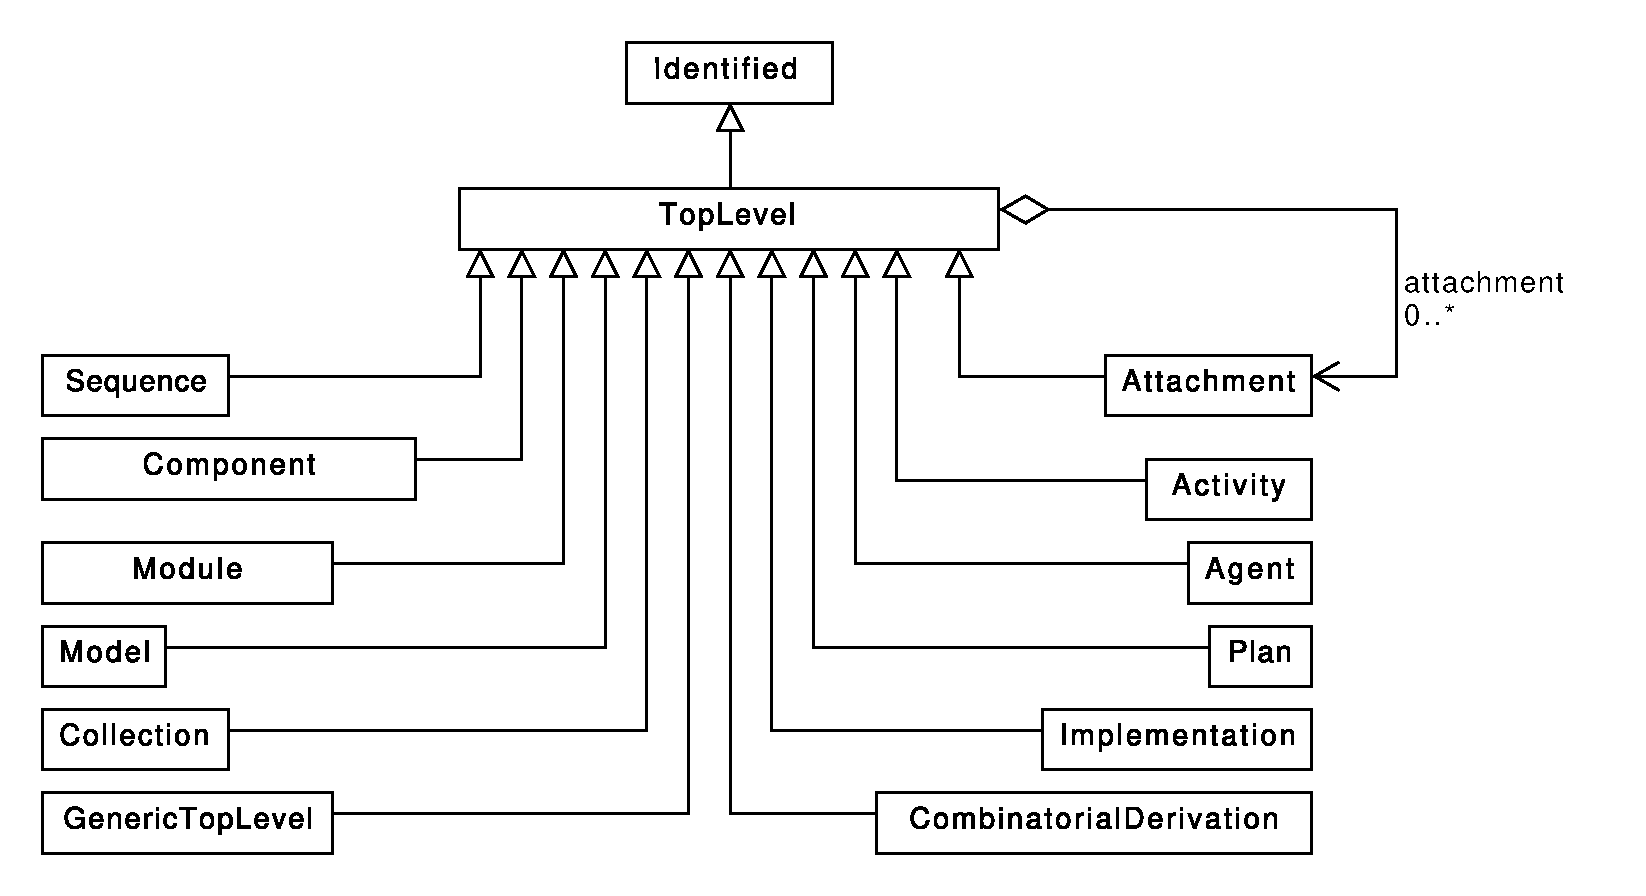
\includegraphics[width=\textwidth]{uml/toplevel}
\caption[]{The TopLevel classes}
\label{uml:toplevel}
\end{center}
\end{figure}




\subsection{Sequence}
\label{sec:Sequence}
The Sequence class is used to encode the primary structure of a ComponentDefinition object using a String of characters. Sequence objects identify their type of encoding with a URI. For example, a Sequence object that encodes a DNA sequence would have an IUPAC DNA encoding, while a Sequence object that encodes the chemical structure of glucose might have a simplified molecular-input line-entry system (SMILES) encoding. 

\begin{figure}[ht]
\begin{center}
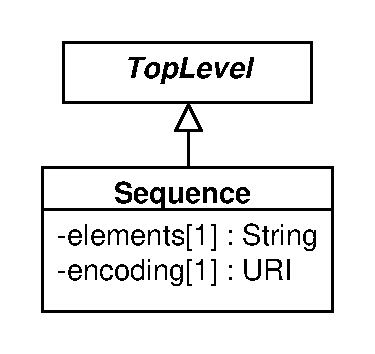
\includegraphics[scale=0.6]{uml/sequence}
\caption[]{Sequence class}
\label{uml:sequence}
\end{center}
\end{figure}




\subsection{ComponentDefinition}
\label{sec:ComponentDefinition}
The proposed Version 2.0 data model generalizes the DnaComponent class of SBOL Version 1.1 to a Component class in order to support an increased range of structural representation. Components can represent genetic components such as DNA, but also RNA and proteins which were unrepresented in Version 1.1.  Additionally, the generalized Component class can even represent non-genetic components, such as non-biological polymers, small molecules, molecular complexes, and even light.

% Figure has some classes named incorrectly
\begin{figure}[ht]
\begin{center}
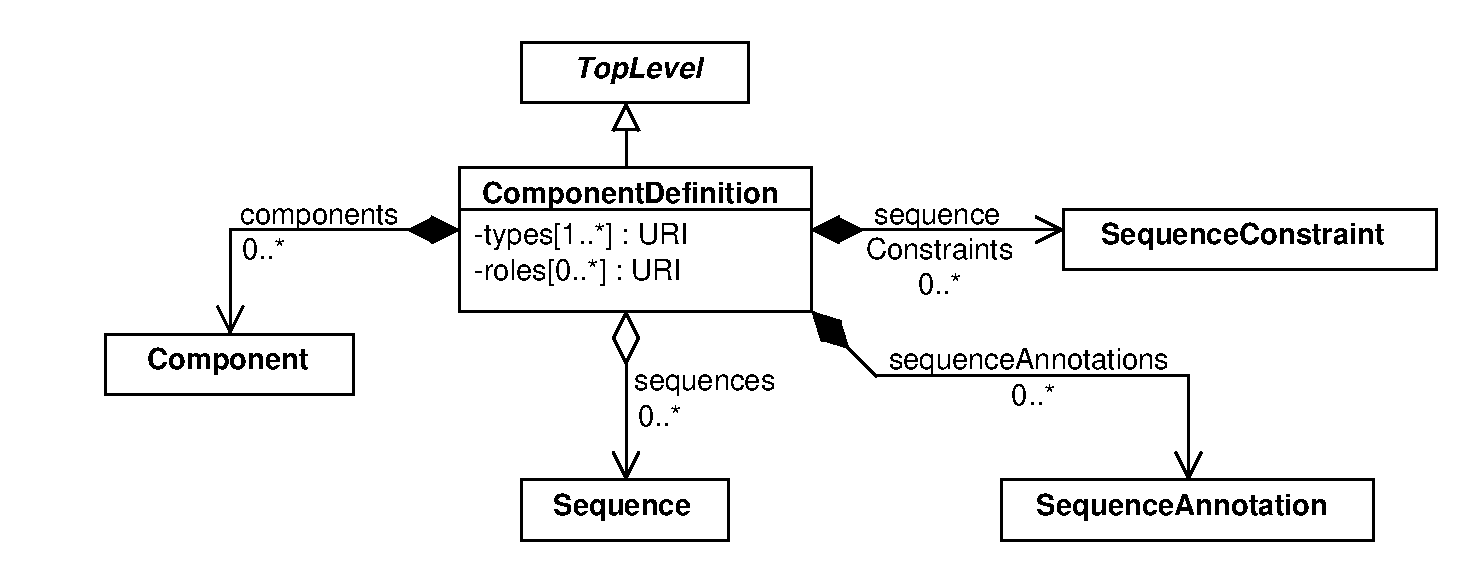
\includegraphics[width=\textwidth]{uml/component_definition}
\caption[]{ComponentDefinition}
\label{uml:component_definition}
\end{center}
\end{figure}

Another significant change is that a layer of design abstraction has been added to the Component class.  The ComponentDefinition base class is analagous to a blueprint or parts specification sheet for a biological part.  In contrast, the Component class represents specific occurrences of a part within a design.  Thus the new version of SBOL supports biological designs that re-use the same component more than once. 

% Examples of ontologies for non-molecular type ComponentDefinitions (eg, light)...?
A ComponentDefinition which contains the blueprint for a molecular component must have at least one type URI that identifies a term from an appropriate ontology, such as the ontology of Chemical Entities of Biological Interest (ChEBI) and the BioPAX ontology. A type URI documents the basic sort of biochemical or physical entity (for example DNA, protein, or RNA) that a Component object abstracts for the purpose of engineering design. If a Component object has multiple type URIs, then they must identify synonymous terms.
\textcolor{red}{Examples of ontologies for non-molecular type ComponentDefinitions (eg, light)...?}

The roles of a ComponentDefinition object, on the other hand, are analogous to the type of a DnaComponent object in SBOL Version 1.1 and the sequence types of a SequenceComponent in the ACS Synthetic Biology paper. Role URIs are expected to identify ontology terms that clarify a Component object’s potential function in a biological context. For example, a ComponentDefinition object of type “DNA” may have a role of “promoter” or “terminator,” terms taken from the Sequence Ontology (SO). A ComponentDefinition object of type “protein,” on the other hand, may have a role of “transcription factor” or “protease.” 

% Are the class names listed here correct, taking recent name changes into account?
\textcolor{red}{Finally, a ComponentDefinition object can define its structure by linking to objects that belong to the StructuralInstance, Sequence, SequenceAnnotation, and SequenceConstraint classes. These classes are described below.}

\subsubsection{SequenceAnnotation}
\label{sec:SequenceAnnotation}
The SequenceAnnotation class describes a location of interest on the Sequence object linked by its parent ComponentDefinition object and may optionally associate this location with a StructuralComponent object. SequenceAnnotation objects pecify their location using a Location object. As explained below, the Location class is extended by several different classes, some of which assert locations other than simple ranges with start and end positions.

\begin{figure}[ht]
\begin{center}
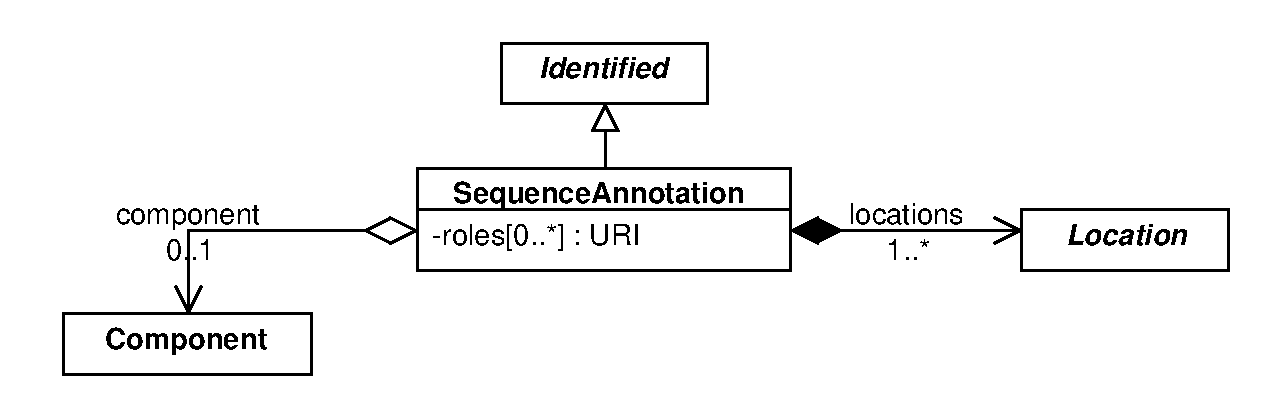
\includegraphics[scale=0.6]{uml/sequence_annotation}
\caption[]{SequenceAnnotation class}
\label{uml:sequence_annotation}
\end{center}
\end{figure}




\subsubsection{SequenceConstraint}
\label{sec:SequenceConstraint}
In SBOL Version 1.1 partial designs are made possible by means of SequenceAnnotation objects that can specify that their locations precede those of other SequenceAnnotation objects. In Version 2.0 the “precedes” data field has been generalized to the StructuralConstraint class. A ComponentDefinition object can link to SequenceConstraint objects to assert different kinds of structural restrictions (not just precedes relationships) between the StructuralComponent objects that represent its subcomponents. These restrictions could include “sameOrientationAs” or “oppositeOrientationAs” to enable the relative orientation of StructuralComponent objects whose ComponentDefinition objects lack associated Sequence objects in partial designs.

\begin{figure}[ht]
\begin{center}
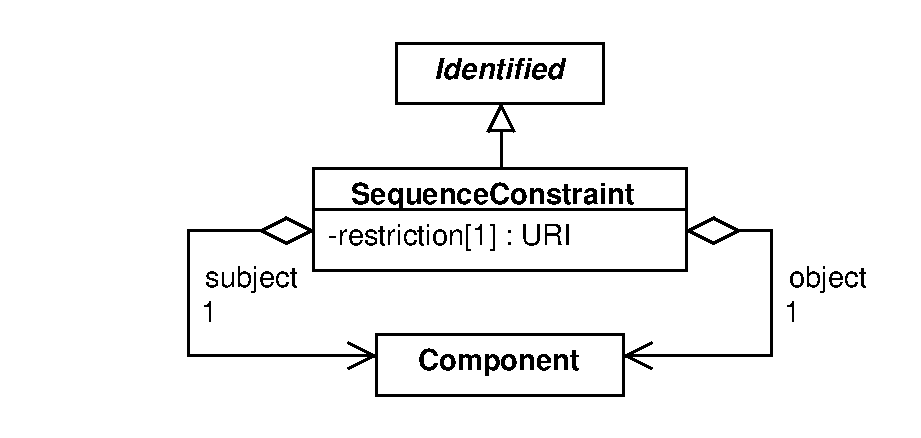
\includegraphics[scale=0.6]{uml/sequence_constraint}
\caption[]{SequenceConstraint class}
\label{uml:sequence_constraint}
\end{center}
\end{figure}




\subsubsection{Location}
\label{sec:Location}
The Location class is extended by the Range, MultiRange, and Cut classes, and the Range and Cut classes are further extended by the OrientedRange and OrientedCut classes. First, a Range object specifies inclusive start and end positions greater than zero, while an OrientedRange object includes an “orientation” data field suitable for specifying locations on a potentially double-stranded Component object.

\begin{figure}[ht]
\begin{center}
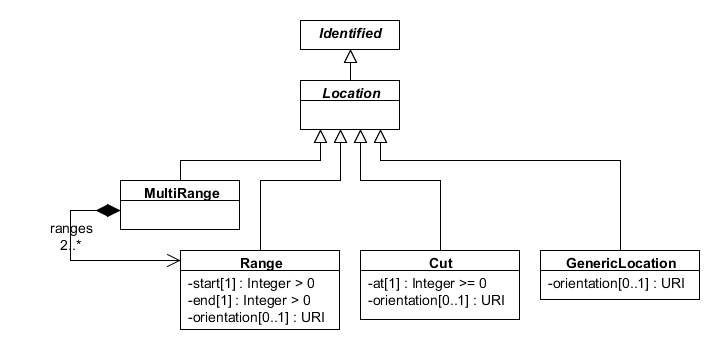
\includegraphics[scale=0.6]{uml/location}
\caption[]{Location class}
\label{uml:location}
\end{center}
\end{figure}

Second, A MultiRange object represents a location that is specified by multiple Range objects. For example, this capability can be used to specify a ComponentDefinition object that represents the introns or exons of a eukaryotic gene.

Third, the Cut class has been introduced to enable the specification of a location between two indices. Each Cut object has a single integer data field, “at,” that specifies the index just before the location represented by the Cut object. Even though there is no zero index on Structure objects in SBOL, a Cut object with “at” equal to zero represents the location just before index one. The OrientedCut class extends the Cut class with an orientation in the same way that the OrientedRange class extends the Range class.

Finally, while the Range and Cut classes are best suited to describing locations on sequential structures, the Location class can be extended in the future to better describe locations on Component Objects with non-sequential structure (see unspecified Moeity class as potential means for specifying locations in more than one dimension).




\subsubsection{ComponentInstance}
\label{sec:ComponentInstance}

\begin{figure}[ht]
\begin{center}
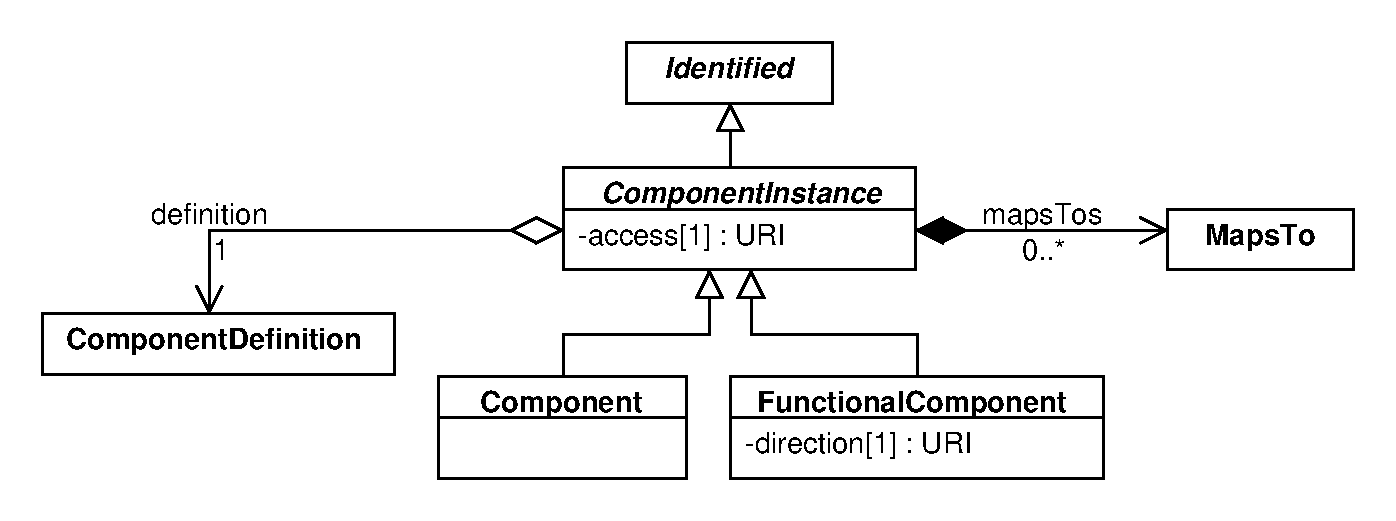
\includegraphics[scale=0.6]{uml/component_instance}
\caption[]{Component}
\label{uml:component}
\end{center}
\end{figure}

% The second sentence is confusing.
Hierarchical compositions of structure and function is enabled via the ComponentInstance class. Each ComponentInstance object has three data fields. \textcolor{red}{The first data field, “definition”, links to the Component object that is effectively a part of the Component or Module object that owns the ComponentInstantiation object.} The second data field, “access,” defines whether the ComponentInstance object can be referred to by ComponentInstance objects that are higher in the design hierarchy (yes if access is set to “public”). The third data field, "mappings", is a set of MapsTo objects that link between other ComponentInstance objects at the same level of the design hierarchy as well as other ComponentInstance objects that are lower in the design hierarchy, thereby composing these objects with greater specificity (see first module example).

There are two subclasses of the ComponentInstance class: the StructuralComponent and FunctionalComponent classes.




\subsubsection{Component}
\label{sec:Component}
Composition of the structural layer of SBOL designs is accomplished using StructuralInstance objects. Each StructuralComponent object is owned by a ComponentInstance object and serves as an explicit usage of a \textcolor{red}{sub-Component} object for the purpose of physical composition.




\subsubsection{FunctionalComponent}
\label{sec:FunctionalComponent}
Composition of the functional layer of SBOL designs, on the other hand, is accomplished using FunctionalComponent objects. Each FunctionalComponent object is owned by a Module object and serves as an explicit usage of a ComponentInstance object for the purpose of fulfilling some function. In addition, each FunctionalInstantiation must specify via the “direction” field whether it serves as an  input, output, both, or neither for its parent Module object. 




\subsection{ModuleDefinition}
\label{sec:ModuleDefinition}

\begin{figure}[ht]
\begin{center}
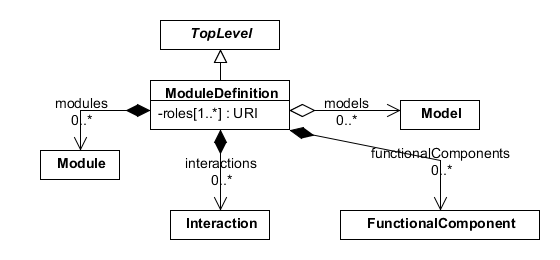
\includegraphics[scale=0.6]{uml/module_definition}
\caption[]{ModuleDefinition}
\label{uml:module_definition}
\end{center}
\end{figure}

The ModuleDefinition class forms the hub for functional description of genetic designs. A Module object is composed from zero or more FunctionalComponent, Module, and Interaction objects, and links to zero or more Model objects. A Module object relies on the “direction” data fields of its FunctionalComponent objects to specify whether they serve as its inputs or outputs.

In addition, each ModuleDefinition object must now have at least one of potentially several roles to indicate its intended usages. For example, the role URIs on a ModuleDefinition object may identify terms for abstract module roles, such as “inverter” or “AND gate,” or they may identify terms for biological module roles, such as “metabolic pathway” and “signaling cascade.”




\subsubsection{Module}
\label{sec:Module}

\begin{figure}[ht]
\begin{center}
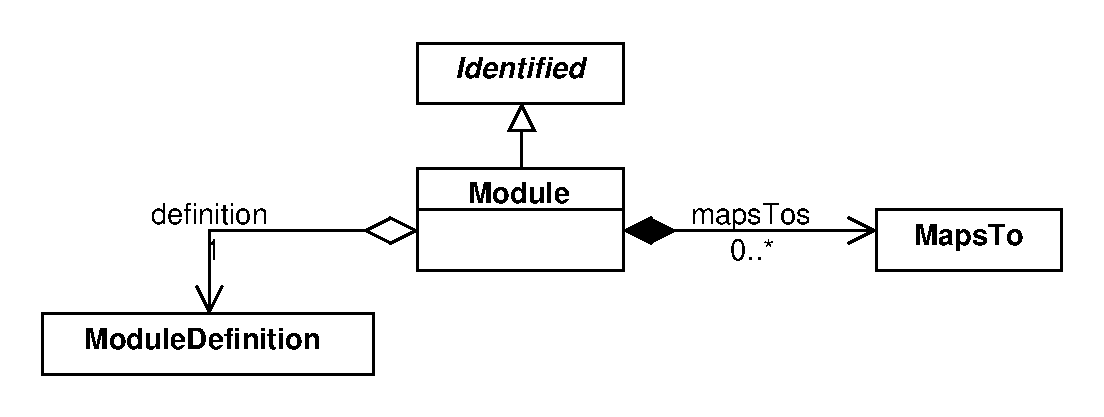
\includegraphics[scale=0.6]{uml/module}
\caption[]{Module}
\label{uml:module}
\end{center}
\end{figure}

The Module class enables the composition of Module objects from other sub-Module objects. \textcolor{red}{The first data field, “definition”, links to the ModuleDefinition object that is effectively a part of the Module object that owns the Module object.} The second data field, “mappings”, is a set of MapsTo objects that link between the Component objects at the same level of the design hierarchy as the Module object and the Component objects that are lower in the design hierarchy, thereby composing these objects with greater specificity.




\paragraph{MapsTo}
\label{sec:MapsTo}

\begin{figure}[ht]
\begin{center}
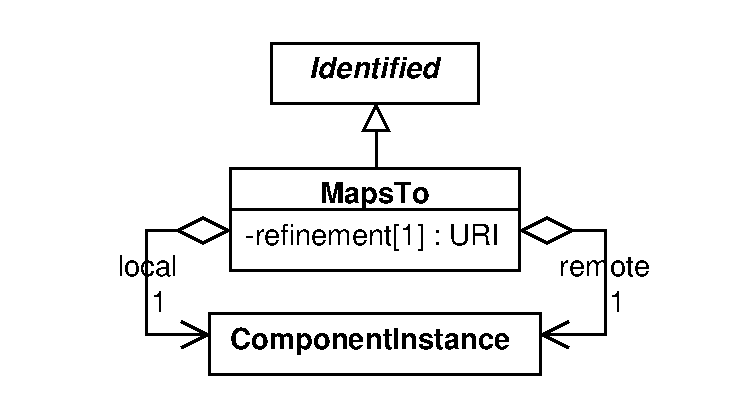
\includegraphics[scale=0.6]{uml/maps_to}
\caption[]{}
\label{uml:maps_to}
\end{center}
\end{figure}
The MapsTo class serves as a means of linking between Component objects (both StructuralComponents and FunctionalComponents) at different levels of the design hierarchy. For example, when a Module object is instantiated inside another Module object, a MapsTo object on the appropriate Module  object can be used to link between a FunctionalComponent object in the parent Module (as specified by the “local” data field) and a FunctionalComponent object in the child module (as specified by the “remote” data field). This linking can perhaps be most easily understood via the examples in the next section.

In addition to specifying a link, each MapsTo object must also specify a “refinement” relationship between its local and remote Components. Under this data model, there are four types of refinement: “verifyIdentical” requires that the Component objects link to the same ComponentDefinition object, “useLocal” indicates that the local Component object overrides the remote Component object, “useRemote” indicates the opposite, and “merge” indicates that data fields of the local and remote ComponentInstantiation objects are to be interpreted in combination.


\subsubsection{Interaction}
\label{sec:Interaction}

\begin{figure}[ht]
\begin{center}
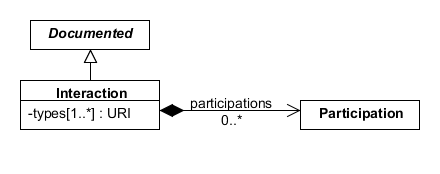
\includegraphics[scale=0.6]{uml/interaction}
\caption[]{Interaction}
\label{uml:interaction}
\end{center}
\end{figure}

The Interaction class provides a qualitative basis for asserting the intended function of a given ModuleDefinition object. The proposed data model supports the representation of regulatory interactions, such as activation or repression, and processes from the central dogma of biology, such as transcription and translation. Other supported interaction types include non-covalent binding between a small molecule and TF, and phosphorylation of a TF by an enzyme. 

Each Interaction object must specify its type with at least one URI that identifies an appropriate ontology term, such as a term from the Systems Biology Ontology (SBO). If an Interaction object has multiple type URIs, then they must identify synonymous terms. 

Furthermore, each Interaction object must specify its participating ComponentInstantiation objects by linking to one or more objects of the Participation class.

\begin{figure}[ht]
\begin{center}
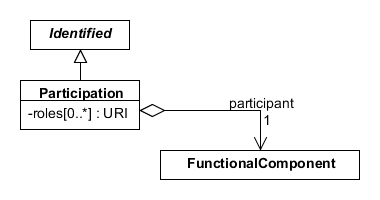
\includegraphics[scale=0.6]{uml/participation}
\caption[]{Participation}
\label{uml:participation}
\end{center}
\end{figure}

\subsubsection{Participation}
\label{sec:Participation}
Each object of the Participation class must specify the role of its participant FunctionalComponent object in its parent Interaction object with at least one URI that identifies an appropriate ontology term. If a Participation object has multiple role URIs, then they must identify synonymous terms. 

While the Interaction class provide a qualitative description of genetic function, quantitative descriptions are also needed for genetic design. Instead of introducing a new language for the specification of mathematical models of biology, the proposed data model leverages existing standards and links to them via the Model class. 




\subsection{Model}
\label{sec:Model}

\begin{figure}[ht]
\begin{center}
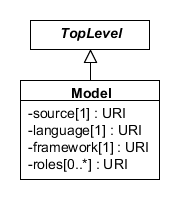
\includegraphics[scale=0.6]{uml/model}
\caption[]{}
\label{uml:model}
\end{center}
\end{figure}

Each Model object is required to link by means of URIs to a source model and ontology terms that identify the source model's language, framework, and potential roles (multiple). In this way, there is minimal duplication of standardization efforts and users of SBOL can specify the quantitative function of their ModuleDefinition objects in a well-developed language of their choice. A ModuleDefinition object can link to more than one model since each one can encode different levels of functional detail and play different roles in engineering design. 




\subsection {Collection}
\label{sec:Collection}
The \sbol{Collection} class is another top level class, which groups together \sbol{TopLevel} objects that have something in common. For example, a \sbol{Collection} object could be the result of a query to find all \sbol{Component} objects that function as promoters or all \sbol{Module} objects that function as inverters in a given repository. The example in \ref{ser:Collection} shows the serialisation of a \sbol{Collection} object. 

\begin{figure}[ht]
\begin{center}
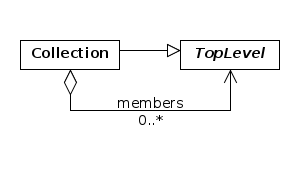
\includegraphics[scale=0.6]{uml/collection}
\caption[]{The Collection class}
\label{uml:collection}
\end{center}
\end{figure}

\begin{figure} [ht]
\lstsetsbol
\begin{lstlisting}
  <sbol:Collection rdf:about="http://sbols.org/v2#col1">
    <sbol:timeStamp>2015-02-16 16:37:54.381</sbol:timeStamp>
    <sbol:displayId>col1</sbol:displayId>
    <sbol:name>Collection 1</sbol:name>
    <sbol:description>A colleciton of DNA components</sbol:description>
    <sbol:member rdf:resource="http://sbols.org/v2#com2"/>
    <sbol:member rdf:resource="http://sbols.org/v2#com1"/>
    ...
</sbol:Collection>
\end{lstlisting}
\label{ser:Collection}
\end{figure}




\subsection{Application Specific Data - Annotations}
\label{sec:annotations}


\subsubsection{Annotating SBOL objects}
SBOL allows embedding application specific data that are not captured by the SBOL standard. Such data are optional, can be computationally generated and exchanged via SBOL documents without getting lost. These custom data are stored in the form of annotations, providing informative metadata about entities in an SBOL document.

Each \sbol{Identified} object may have a number of annotations in the form of name/value property pairs. Property names are specified by qualified names as \external{IRI}s, each formed of a namespace and a local name. Values can be \external{IRI}s or \external{Literal}s (for example, \external{String}, \external{Integer}, \external{Double}, \external{Boolean}) or custom \sbol{identity} entities initialized with application specific types. These custom \sbol{identity} entities can further be annotated with the scheme described here. These custom entities are either serialized within an SBOL entity being annotated, or referenced using an \external{IRI} annotation and embedded within the the annotated entity's parent.%TODO Make sure if we have a choice here! 

\begin{figure}[!ht]
\begin{center}
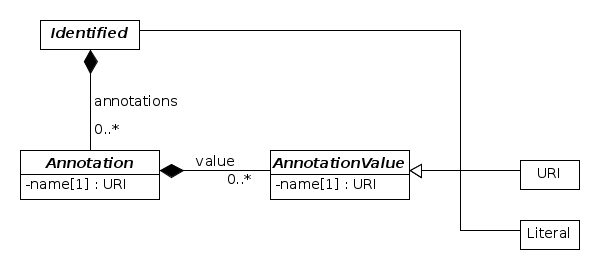
\includegraphics[scale=0.6]{uml/identified_annotations}
\caption[]{Annotating SBOL's Identified entities with application specific data.}
\label{uml:identified_annotations}
\end{center}
\end{figure}

  Each annotation is serialised as an RDF subject-property-object triplet in which the subject is the SBOL object being annotated, the property is the annotation name, and the object is the annotation value. Simple values URIs are serialised as RDF literals, and URI values are represented with the \external{\path{http://www.w3.org/1999/02/22-rdf-syntax-ns#resource}} RDF property. If the annotation value is another complex object then the object is embedded as an RDF resource, which can further be annotated similarly.%TODO If we allow URI reference of a custom object stored, then update this paragraph

The ComponentDefinition example for a promoter below shows how annotations can be added to SBOL objects. Annotations are added using the relevant information from the Parts Registry. Annotation property names are qualified with the \external{http://www.partsregistry.org/} namespace, which is prefixed using \external{pr}. The first annotation is named as \external{pr:group}, indicating the iGEM group designing the promoter, and has a \external{String} value. The second \external{pr:experience} annotation has a \external{URI} value and is serialised as an RDF resource pointing to the information Web page on the Parts Registry for the promoter. The  \external{pr:information} property represents a complex annotation which is a type of \external{pr:Information} and includes information about the regulatory details of the promoter using Parts Registry categories.   

\begin{figure} [ht]
\lstsetsbol
\begin{lstlisting}
<?xml version="1.0" ?>
<rdf:RDF xmlns:rdf="http://www.w3.org/1999/02/22-rdf-syntax-ns#" xmlns:pr="http://www.partsregistry.org/" xmlns:sbol="http://sbols.org/v2#">
  <sbol:ComponentDefinition rdf:about="http://www.partsregistry.org/Part:BBa_J23119">
    <pr:group>iGEM2006_Berkeley</pr:group>
    <pr:experience rdf:resource="http://www.partsregistry.org/Part:BBa_J23119:Experience"/>
    <pr:information>
      <pr:Information rdf:about="http://parts.igem.org/cgi/partsdb/part_info.cgi?part_name=BBa_J23119">
        <pr:sigmafactor>//rnap/prokaryote/ecoli/sigma70</pr:sigmafactor>
        <pr:regulation>//regulation/constitutive</pr:regulation>
      </pr:Information>
    </pr:information>
    <sbol:name>J23119</sbol:name>
    <sbol:description>Constitutive promoter</sbol:description>
    <sbol:type rdf:resource="http://www.biopax.org/release/biopax-level3.owl#DnaRegion"/>
    <sbol:role rdf:resource="http://purl.org/obo/owl/SO#SO_0000167"/>
  </sbol:ComponentDefinition>
</rdf:RDF>
\end{lstlisting}
\label{ser:Annotation}
\end{figure}




\subsubsection{GenericTopLevel}  
\label{sec:GenericTopLevel}
SBOL documents can also be annotated at the top level. SBOL's \sbol{GenericTopLevel} is a top-level entity that can include a set of annotations as described above. Entities that are at the top-level and are not recognised by the SBOL standard are loaded into these top level entities. These \sbol{GenericTopLevel} entities may have multiple type information and can be used safely by tools to exchange custom data. As with any other top level entities, \sbol{GenericTopLevel} entities may include SBOL properties such as \sbol{name}, \sbol{description}, \sbol{displayId} and so on.
%TODO: Is it possible to have multiple types for GenericTopLevel elements? If so, update the diagram.

\begin{figure}[ht]
\begin{center}
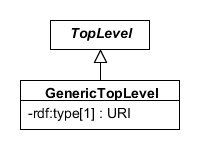
\includegraphics[scale=0.6]{uml/generictoplevel}
\caption[]{Annotating SBOL documents with GenericTopLevel entities.}
\label{uml:generictoplevel}
\end{center}
\end{figure}

The example below shows adding a datasheet object to a SBOL document using the \sbol{GenericTopLevel} class. The J23119 promoter example is annotated with the URI of a top Level Datasheet object. The annotation properties are defined using the custom \external{\path{http://www.myapp.org/}} namespace and the \external{myapp} prefix. The datasheet object, with the data type of \external{myapp:Datasheet}, is accessed using the \external{URI} value specified by the \external{myapp:characterizationData} property of the promoter component definition. The datasheet object is further annotated with the transcription rate and the URI for the actual characterization data using the \external{myapp:transcriptionRate} and \external{myapp:characterizationData} properties respectively.

\begin{figure}[ht]
\lstsetsbol
\begin{lstlisting}
<?xml version="1.0" ?>
<rdf:RDF xmlns:rdf="http://www.w3.org/1999/02/22-rdf-syntax-ns#" xmlns:myapp="http://www.myapp.org/" xmlns:sbol="http://sbols.org/v2#">
  <sbol:ComponentDefinition rdf:about="http://www.partsregistry.org/Part:BBa_J23119">
    <myapp:datasheet rdf:resource="http://www.myapp.org/datasheet/1"/>
    <sbol:name>J23119</sbol:name>
    <sbol:description>Constitutive promoter</sbol:description>
    <sbol:type rdf:resource="http://www.biopax.org/release/biopax-level3.owl#DnaRegion"/>
    <sbol:role rdf:resource="http://purl.org/obo/owl/SO#SO_0000167"/>
  </sbol:ComponentDefinition>
  <myapp:Datasheet rdf:about="http://www.myapp.org/datasheet/1">
    <myapp:characterizationData rdf:resource="http://www.myapp.org/measurement/1"/>
    <myapp:transcriptionRate>1</myapp:transcriptionRate>
    <sbol:name>Datasheet 1</sbol:name>
  </myapp:Datasheet>
</rdf:RDF>

\end{lstlisting}
\label{ser:GenericTopLevel}
\end{figure}




% -----------------------------------------------------------------------------
\section{Examples of Data Model}
\label{sec:examples}
% -----------------------------------------------------------------------------



% -----------------------------------------------------------------------------
\section{Examples of Serialization}
% -----------------------------------------------------------------------------

% -----------------------------------------------------------------------------
\section{Best Practices}
\label{sec:bestpractices}
% -----------------------------------------------------------------------------
Currently, if a developer wishes to change a SBOL object that has been published to the Web, then as a best practice they should create a copy of the SBOL object that incorporates the change, but has a new URI. This practice, however, does not inherently involve a standardized declaration that the second object is a version of the first. Consequently, the ``persistentIdentity'', ``version'', and ``timeStamp'' data fields have been created to provide developers with the means to declare that a set of SBOL objects are versions of each other (by virtue of having the same persistent URI) and label these objects with version Strings and times of creation.


\end{document}


% -----------------------------------------------------------------------------
\section{Authors' Contact Information}
% -----------------------------------------------------------------------------

% For now, this section contains examples of potentially useful code for formatting tables, bullets, etc.

\begin{table}[hb]
  \begin{edtable}{tabular}{ll}
    \toprule
    \textbf{Item} & \textbf{Location} \\
    \midrule
    Distribution archive & \url{\distURL}\\
    Web page		 & \url{\webURL}\\
    Source tree (SVN)    & \url{\srcURL}\\
    \bottomrule
  \end{edtable}
  \caption{Where to find \sbmlpkg on the Internet.}
  \label{where}
\end{table}

\begin{table}[htb]
  \rowcolors{2}{sbmlrowgray}{}
  \renewcommand{\arraystretch}{1.05}
  \begin{edtable}{tabular}{ll}
    \toprule
    \textbf{Command}                      & \textbf{Object} \\
    \midrule
    \cmd{AlgebraicRule}                   & \AlgebraicRule \\
    \cmd{Annotation}                      & \Annotation \\
    \cmd{AssignmentRule}                  & \AssignmentRule \\
    \cmd{Compartment}                     & \Compartment \\
    \cmd{Constraint}                      & \Constraint \\
    \cmd{Delay}                           & \Delay \\
    \cmd{EventAssignment}                 & \EventAssignment \\
    \cmd{Event}                           & \Event \\
    \cmd{FunctionDefinition}              & \FunctionDefinition \\
    \cmd{InitialAssignment}               & \InitialAssignment \\
    \cmd{KineticLaw}                      & \KineticLaw \\
    \cmd{ListOfCompartments}              & \ListOfCompartments \\
    \cmd{ListOfConstraints}               & \ListOfConstraints \\
    \cmd{ListOfEventAssignments}          & \ListOfEventAssignments \\
    \cmd{ListOfEvents}                    & \ListOfEvents \\
    \cmd{ListOfFunctionDefinitions}       & \ListOfFunctionDefinitions \\
    \cmd{ListOfInitialAssignments}        & \ListOfInitialAssignments \\
    \cmd{ListOfLocalParameters}           & \ListOfLocalParameters \\
    \cmd{ListOfModifierSpeciesReferences} & \ListOfModifierSpeciesReferences \\
    \cmd{ListOfPackages}                  & \ListOfPackages \\
    \cmd{ListOfParameters}                & \ListOfParameters \\
    \cmd{ListOfReactions}                 & \ListOfReactions \\
    \cmd{ListOfRules}                     & \ListOfRules \\
    \cmd{ListOfSpeciesReferences}         & \ListOfSpeciesReferences \\
    \cmd{ListOfSpecies}                   & \ListOfSpecies \\
    \cmd{ListOfUnitDefinitions}           & \ListOfUnitDefinitions \\
    \cmd{ListOfUnits}                     & \ListOfUnits \\
    \cmd{LocalParameter}                  & \LocalParameter \\
    \cmd{Message}                         & \Message \\
    \cmd{Model}                           & \Model \\
    \cmd{ModifierSpeciesReference}        & \ModifierSpeciesReference \\
    \cmd{Notes}                           & \Notes \\
    \cmd{Package}                         & \Package \\
    \cmd{Parameter}                       & \Parameter \\
    \cmd{Priority}                        & \Priority \\
    \cmd{RateRule}                        & \RateRule \\
    \cmd{Reaction}                        & \Reaction \\
    \cmd{Rule}                            & \Rule \\
    \cmd{SBML}                            & \SBML \\
    \cmd{SBase}                           & \SBase \\
    \cmd{SimpleSpeciesReference}          & \SimpleSpeciesReference \\
    \cmd{SpeciesReference}                & \SpeciesReference \\
    \cmd{Species}                         & \Species \\
    \cmd{StoichiometryMath}               & \StoichiometryMath \\
    \cmd{Trigger}                         & \Trigger \\
    \cmd{UnitDefinition}                  & \UnitDefinition \\
    \cmd{Unit}                            & \Unit \\
    \bottomrule
  \end{edtable}
  \caption{Commands for the names of object classes defined in the SBML Level~3
    Core specification.} 
  \label{sbmlcore}
\end{table}

\begin{example}[style=latex]
\documentclass{sbmlpkgspec}
\begin{document}

\packageTitle{Example}
\packageVersion{Version 1 (Draft)}
\packageVersionDate{14 August 2011}
\packageGeneralURL{http://sbml.org/Documents/Specifications/Example}
\packageThisVersionURL{http://sbml.org/Documents/Specifications/Example_14_August_2011}

\author{Michael Hucka\\[0.25em]
  \mailto{mhucka@caltech.edu}\\[0.25em]
  Computing and Mathematical Sciences\\
  California Institute of Technology\\
  Pasadena, CA, USA
}

\maketitlepage
\maketableofcontents

\section{...}
...
\end{document}
\end{example}


\begin{description}[font=\normalfont\ttfamily\color{black},style=nextline]

\item[draftspec] This option causes the front page of the document to contain
  the word ``DRAFT'' in large gray letters, and the footer of every page of
  the document to contain the word ``(DRAFT)''.  Authors should use this
  option until such time as the specification document is considered a
  release candidate or a final release.

\end{description}

\begin{description}

\item[\hspace*{6.5pt}\vSymbol\vsp] A \vSymbolName indicates a
  \emph{requirement} for conformance. If a model fails to follow this rule,
  it does not conform to the specification.  (Mnemonic intention behind the
  choice of symbol: ``This must be checked.'')

\item[\hspace*{6.5pt}\cSymbol\csp] A \cSymbolName indicates a
  \emph{recommendation} for model consistency.  If a model does not follow
  this rule, it is not considered strictly invalid as far as the
  specification is concerned; however, it indicates that the model contains
  a physical or conceptual inconsistency.  (Mnemonic intention behind the
  choice of symbol: ``This is a cause for warning.'')

\item[\hspace*{6.5pt}\mSymbol\msp] A \mSymbolName indicates a strong
  recommendation for good modeling practice.  This rule is not
  strictly a matter of SBML encoding, but the recommendation comes
  from logical reasoning.  As in the previous case, if a model does
  not follow this rule, it is not strictly considered an invalid SBML
  encoding.  (Mnemonic intention behind the choice of symbol: ``You're
  a star if you heed this.'')

\end{description}

\begin{itemize}

\item \texttt{amssymb}: This package defines many symbols and special
  characters.  In \sbmlpkg, it is used to get the symbols defined by the
  validation rule commands \cmd{validRule}, \cmd{consistencyRule} and
  \cmd{modelingRule} described in \sec{validation-rules}.

\end{itemize}

%\clearpage
%\bibliography{sbmlpkgspec}

% -----------------------------------------------------------------------------
% End of document
% -----------------------------------------------------------------------------

\end{document}
%
% 
%